\item \points{2b} {\bf Degree-3 polynomial regression}


For this sub-question question, we will use the datasets provided in
the following file:
%
\begin{center}
	\texttt{src/train.csv}
\end{center}
%

This file contains two columns: $x$ and $y$. In the terminology described in the introduction, $x$ is the attribute (in this case one dimensional) and $y$ is the output label.

Using the formulation of the previous sub-question, implement linear regression with \textbf{normal equations} using the feature map of degree-3 polynomials. Using the |LinearModel| provided in |src/submission.py|, this means you will be implementing the functions |fit()|, |predict()|, and |create_poly()|.  

To verify a correct implementation, autograder test case |2b-2-basic| will create a plot in |src/large-poly3.png|.  This plot should look similar to the following:
\begin{figure}[H]
  \centering
  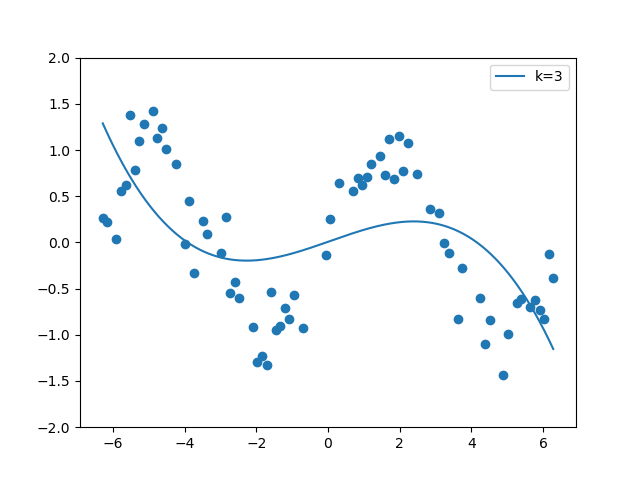
\includegraphics[width=0.65\linewidth]{02-featuremaps/large-poly3.png}
  \centering
\caption{Polynomial regression with degree 3}
\end{figure}

\emph{Remark: } Suppose $\widehat{X}$ is the design matrix of the transformed dataset. You may sometimes encounter a non-invertible matrix $\widehat{X}^T\widehat{X}$. For a numerically stable code implementation, always use \texttt{np.linalg.solve} to obtain the parameters directly, rather than explicitly calculating the inverse and then multiplying it with $\widehat{X}^Ty$.
